\subsection{Experiment Interfaces}

\subsubsection{Mechanical Interfaces}
\label{sec:4.2.1}
The experiment box will be fixed to the gondola rails by means of eight brackets, as seen in Figure \ref{fig:bracket}, interfacing the experiment outside structure with the hammer nuts in the rails. This method is secure as well as fast enough to provide an accessible and easy recovery for later analysis.

\begin{figure}[H]
    \centering
    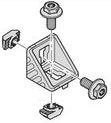
\includegraphics[width=0.2\textwidth]{4-experiment-design/img/Mechanical/bracket.jpg}
    \caption{Bracket Component}
    \label{fig:bracket}
\end{figure}

A simple but reliable fixing interface between the two boxes of the experiment has been designed to ensure the fast recovery of the CAC box. The latter implies only unscrewing 12 bolts as well as unplugging a D-Sub connector. Once the CAC box is detached, the AAC Box will still remain perfectly fixed in the gondola. Table \ref{table:attaching-components} gathers up all the components required to fix the experiment to the gondola. 

\begin{table}[H]
\noindent\makebox[\columnwidth]{%
\scalebox{0.8}{
\begin{tabular}{|c|c|c|c|c|c|}
\hline
\textbf{Component} & \textbf{Interface} & \textbf{Amount} & \textbf{Dimensions} &  \begin{tabular}[c]{@{}c@{}}\textbf{Total}\\ \textbf{weight}\end{tabular}  \\ \hline
Bracket standard 20/20 slot 6/6 & AAC-Gondola & $8$ & $20 \times 20 \times 20\ mm$ & $40\ g$ \\ \hline
Tolerance holes bracket & CAC-Gondola & $2$ & $ 20 \times 30 \times 52 \ mm$ & $50\ g$ \\ \hline
4-hole plate & AAC-CAC & $6$ & $1 \times 60 \times 45\ mm$ & $100\ g$ \\ \hline
Rubber bumpers M6 & AAC-Gondola, CAC-Gondola & $10$ & $19 \times 19 \times 15\ mm$ & $300\ g$ \\ \hline
T-nut slot 6 M4 & AAC-CAC, AAC-Gondola, CAC-Gondola & $44$ & $4 \times 5.9 \times 11.5\ mm$ & $132\ g$ \\ \hline
T-nut slot 8 M6 & AAC-Gondola, CAC-Gondola & $10$ & $6 \times 11 \times 16\ mm$ &  $60\ g$ \\ \hline

Steel bolt M4 & AAC-CAC, AAC-Gondola & $44$ & $8\ mm $ length & $34\ g$ \\ \hline
Steel washer M4 & AAC-CAC, AAC-Gondola & $24$ &\begin{tabular}[c]{@{}c@{}}$ID=4.3\ mm$\\ $OD=9\ mm$\end{tabular} &  $4.8\ g$\\ \hline
% Polyamide bolt M4 & Styrofoam-CAC-AAC & $8$ & $20\ mm $ length & $3\ g$ & $24\ g$ \\ \hline
% Polyamide washer M4 & Styrofoam-CAC-AAC & $8$ &\begin{tabular}[c]{@{}c@{}}$ID=4.3\ mm$\\ $OD=25\ mm$\end{tabular} & $4\ g$ & $32\ g$\\ \hline
Styrofoam bars  & AAC-Gondola, CAC-Gondola & $4$ & see Appendix \ref{sec:mech_drawings} & $450\ g$ \\ \hline
Handles  & CAC \& AAC & $4$ & $ 18.6 \times 25.2 \times 112.5 \ mm$ & $80\ g$ \\ \hline
\end{tabular}}}
\caption{Summary of Gondola-AAC-CAC Interfaces Components.}
\label{table:attaching-components}
\end{table}


Top handles will be mounted to facilitate the experiment box manipulation when moving it in and out of the gondola. 
In order to collect reliable air samples, the experiment requires to be mounted at least with one side exposed to the outside. The later will reduce the pipe length used to collect clean air. Three tubes will extend from the experiment box face. One for the CAC sampling and two, input and output, for the AAC sampling. The one-way selected method will provide a proper flushing of the pipe and thus ensure a reliable sampling as explained in Section \ref{Experiment_Setup}.


\pagebreak
\subsubsection{Electrical Interfaces}
\label{sec:4.2.2}

The experiment will connect to the gondola electrically via a 4 pin, male, box mount receptacle MIL - C-26482P series 1 connector with an 8-4 insert arrangement (MS3112E8-4P) \cite{BexusManual}. It will connect to one 28.8 V/1 mA battery pack which consists of eight SAFT LSH20 batteries in series where each has a 5 A fuse\cite{BexusManual}. The expected maximum current is 1.1 A.

\begin{figure}[H]
    \centering
    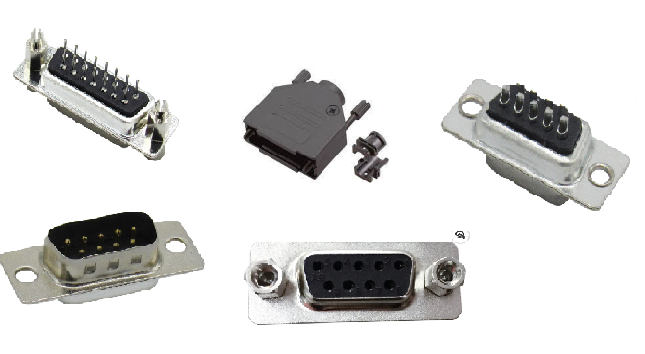
\includegraphics[width=0.4\textwidth]{4-experiment-design/img/connectors.png}
    \caption{Connectors}
    \label{fig:connectors}
\end{figure}

The E-Link connection shall be made between the experiment and the E-Link system using a RJ45 connection which will be supplied by SSC and an Ethernet protocol. The Amphenol RJF21B connector will be mounted on either the front or the side of the experiment\cite{BexusManual}.  

The CAC and AAC will be connected together with a D-SUB 9-pin connector where power, ground and signals for the sensors in the CAC will be connected. A female connector will be located on the AAC wall and a male connector on the CAC wall.

Another female D-SUB 9-pin connector will be located on the wall of the AAC in which the connections for the three ambient pressure sensors will be located. Connectors with different pin configuration are shown in Figure \ref{fig:connectors}.

The expected data rate is 1.58 kbits/s for downlink and 1.08 kbits/s for uplink.

%\begin{figure}[H]
%    \begin{align*}
%        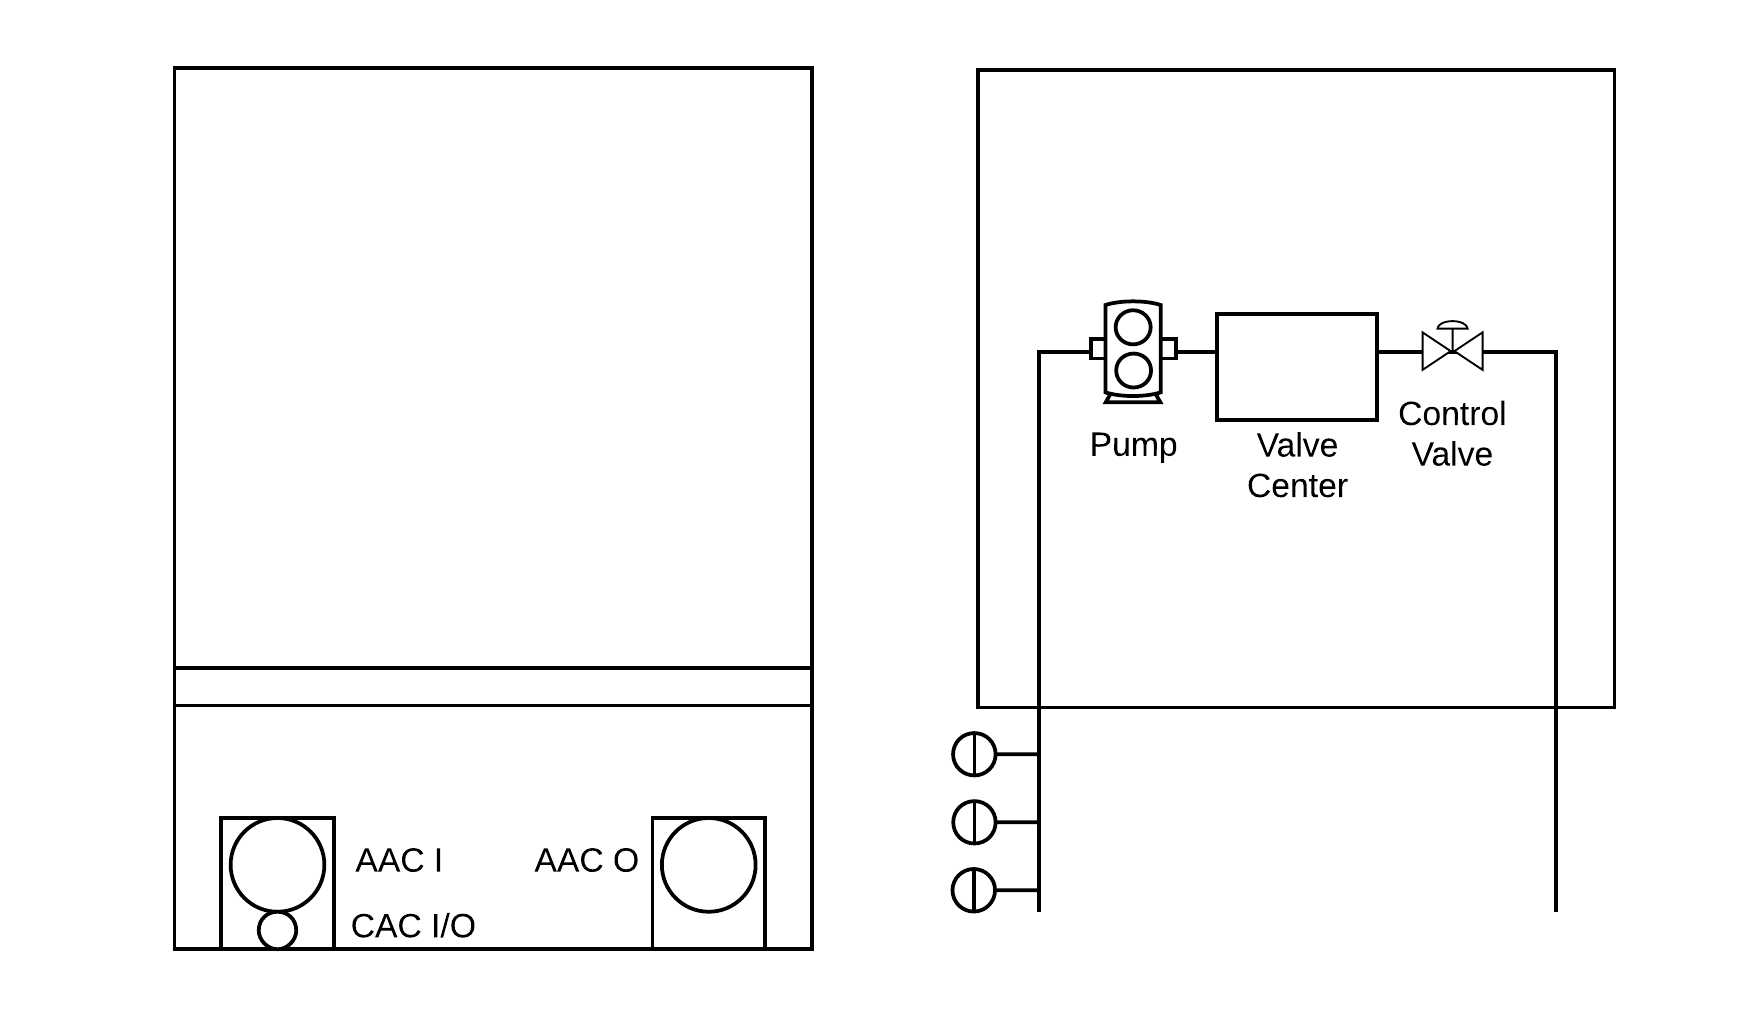
\includegraphics[width=0.7\textwidth]{4-experiment-design/img/Diagram_pipe.png}
%    \end{align*}
%    \caption{Diagram of the experiment box face exposed to the outside.}\label{fig:pipes_interface_1}
%\end{figure}

\iffalse
\subsubsection{Radio Frequencies (Optional)}
\begin{centering}
Not required.
\end{centering}
\bigskip

\subsubsection{Thermal (Optional)}
\begin{centering}
Not required.
\end{centering}
\bigskip
\fi


\raggedbottom